\documentclass[11pt]{article}
\usepackage[margin=1in]{geometry}
\usepackage{amsmath,amssymb,amsthm}
\usepackage{graphicx}
\usepackage{booktabs}
\usepackage{hyperref}
\usepackage{xcolor}
\usepackage{microtype}

\title{\textbf{Paper 35: Geographic Relay Coupling in VCML}\\
\large Gain Quantification, Resonance Condition, and the\\
Reappearance of the Correlation Length at the Inter-Module Scale}

\author{Gabriel Aubin-Moreau}
\date{March 2026}

\begin{document}
\maketitle

\begin{abstract}
Paper V100 established that geographic relay coupling --- having a secondary VCML lattice
(L2) receive waves at the \emph{same spatial positions} as the primary lattice (L1) ---
produces a $3.48\times$ gain in spatial structure ($\mathrm{sg4\_norm}$) over a
position-scrambled control.
Here we quantify the relay gain $G(\mathrm{WR}, N_{\mathrm{zones}})$ across wave
rate (Exp A) and zone count (Exp B), and derive the physical constraints that bound it.
\textbf{Q6 (answered):}
The monotone theory $G = (KN + \mathrm{WR})/(K + \mathrm{WR})$ is wrong in kind ---
$G$ is resonant, not monotone, in both arguments.
The gain peaks at wave rate $\mathrm{WR} \approx 4.8$ ($G = 2.67\times$, Exp A) and
degrades catastrophically above the wave-flux threshold $\Phi = 1$
($\Phi \equiv \mathrm{WR} \cdot r_{\mathrm{wave}} / T_{\mathrm{dur}}$),
reaching $G < 1$ for $\mathrm{WR} \geq 9.6$.
The gain is strongest at $N=2$ ($G = 6.19\times$) and collapses to $G \approx 1$ when
the zone width $z_w < 4\xi$, where $\xi \approx 2.5$ sites is the correlation length
established in Paper~3.
Both thresholds are expressions of the same constraint: $\xi$ is load-bearing at every
scale at which it is probed.
Geographic coupling functions as a \emph{structured attractor selector}: it increases the
probability that L2 locks into the spatially structured basin rather than the unstructured
one, and the relay gain measures this differential basin-selection probability.
\end{abstract}

%--------------------------------------------------------------------
\section{Introduction and Context}
%--------------------------------------------------------------------

The VCML research programme has characterised how spatial structure forms within a
single lattice (Papers 0--33). The question of multi-module coupling --- whether a
secondary module can inherit, amplify, or relay the structure of a primary one ---
was first posed in Paper V100 (the geographic relay experiment), which found a $3.48\times$
gain under geographic coupling.

Paper V100 left three questions open:
\begin{enumerate}
  \item What is $G$ as a function of wave rate WR? Is there an optimal operating point?
  \item What is $G$ as a function of zone count $N_{\mathrm{zones}}$?
    The theory predicted $G \to N$ as $\mathrm{WR} \to 0$, giving monotone scaling.
  \item What physical mechanism sets the gain, and is it connected to known VCML constraints?
\end{enumerate}

This paper answers all three.

\subsection*{Setup and metrics}

Two FastVCML lattices (L1, L2) each occupy the active region $x \in [40, 79]$,
$y \in [0, 39]$ ($N = 1600$ sites each, $\mathrm{HS}=2$, standard V46 parameters).
The GeoHierEnv launcher partitions the active region into $N_{\mathrm{zones}}$ horizontal
zones of width $z_w = 40/N_{\mathrm{zones}}$; each wave is assigned a zone class $c$
(even $c$: suppress, odd $c$: excite, amplitudes $0.25$ and $0.50$).
\begin{itemize}
  \item \textbf{Geo condition:} L2 receives waves at the \emph{same} $(c_x, c_y, c)$ as L1.
  \item \textbf{Ctrl condition:} L2 receives waves at independently sampled positions
    and zone classes.
\end{itemize}
Both conditions use the same wave launch rate WR. The relay gain is
\begin{equation}
  G(\mathrm{WR}, N) = \frac{\overline{\mathrm{sg4\_norm}_{\mathrm{geo}}}}{\overline{\mathrm{sg4\_norm}_{\mathrm{ctrl}}}},
\end{equation}
where the overline denotes the mean over 5 seeds and the last 30 sample windows
($T \in [2700, 3000]$, sampled every 20 steps).
Because VCML has a bimodal attractor (structured vs.\ unstructured), individual seeds
can land in either basin regardless of coupling; $G$ as defined measures the
\emph{differential basin-selection probability} --- the degree to which geographic coupling
biases L2 toward the structured attractor --- weighted by attractor depth.

%--------------------------------------------------------------------
\section{Theory: the Monotone Formula and its Failure}
%--------------------------------------------------------------------

The original theory assumed that ctrl L2 sees a diluted version of the structured
input: each ctrl wave lands in the correct zone with probability $1/N$, so the
effective wave rate for zone structure is $\mathrm{WR}/N$. Mapping $\mathrm{sg4} \sim
\mathrm{WR}/(K + \mathrm{WR})$ and taking the ratio gives
\begin{equation}
  G_{\mathrm{monotone}}(\mathrm{WR}, N) = \frac{K N + \mathrm{WR}}{K + \mathrm{WR}},
  \label{eq:mono}
\end{equation}
which is monotone increasing in both WR and $N$, and asymptotes to $N$ as $\mathrm{WR} \to 0$.
A fit to the data yields $K = 0.20$ (expected $K \sim 23$), and the residuals are
large at every point. The formula fails.

The failure is structural. Equation~\eqref{eq:mono} assumes that the geo/ctrl gap only
narrows from the denominator (information dilution), ignoring two physical ceilings:
\begin{enumerate}
  \item \textbf{Wave-flux saturation.} When $\Phi \equiv \mathrm{WR} \cdot r_{\mathrm{wave}} / T_{\mathrm{dur}} \geq 1$,
    waves land faster than the copy-forward loop can equilibrate the field over one
    footprint radius. The result is synchronized collapse cascades that destroy structure in
    \emph{both} geo and ctrl, but geo's spatially correlated waves produce larger, more
    destructive cascades, making G drop below 1.
  \item \textbf{Zone-boundary bleeding.} When $z_w < 4\xi$, where $\xi \approx 2.5$
    sites is the propagation correlation length (Paper~3), the wave footprint overlaps
    adjacent zones. Both geo and ctrl waves inject zone-class signals into the wrong
    zone sites, homogenising the field and eliminating the geo advantage.
\end{enumerate}
A resonant model replaces the monotone formula. In the WR dimension, the gain is
well-described by a log-Gaussian:
\begin{equation}
  G(\mathrm{WR}) = 1 + A \exp\!\left(-\frac{(\ln \mathrm{WR} - \ln \mathrm{WR}_\star)^2}{2\sigma^2}\right),
  \label{eq:peaked}
\end{equation}
with $\mathrm{WR}_\star \approx 3.5$, $A \approx 9.7$, $\sigma \approx 0.17$.
The resonance window is narrow: $\sigma = 0.17$ in log space corresponds to a factor-of-$1.5$
bandwidth. In the $N$ dimension, $G$ is monotone decreasing above $N_{\mathrm{crit}} = z_w / (4\xi) = 40 / (4 \times 2.5) = 4$, consistent with the observed transition between $N=4$ ($G = 2.67$) and $N=5$ ($G = 1.06$).

%--------------------------------------------------------------------
\section{Experiments}
%--------------------------------------------------------------------

\subsection*{Experiment A: Wave rate sweep ($N_{\mathrm{zones}} = 4$)}

Six wave rates spanning two decades ($\mathrm{WR} \in \{0.6, 1.2, 2.4, 4.8, 9.6, 19.2\}$)
are crossed with two coupling conditions (geo, ctrl) for 5 seeds each (60 runs).
The corresponding wave flux is $\Phi = \mathrm{WR} \times 2 / 15 \in \{0.08, 0.16, 0.32, 0.64, 1.28, 2.56\}$.

\begin{table}[h]
\centering
\caption{Experiment A: relay gain vs.\ wave rate ($N=4$, 5 seeds).}
\label{tab:exp_a}
\begin{tabular}{rrrrr}
\toprule
WR & $\Phi$ & $\overline{\mathrm{sg4n}}_{\mathrm{geo}}$ & $\overline{\mathrm{sg4n}}_{\mathrm{ctrl}}$ & $G$ \\
\midrule
0.6  & 0.08 & 0.156 & 0.157 & 0.998 \\
1.2  & 0.16 & 0.179 & 0.112 & 1.594 \\
2.4  & 0.32 & 0.247 & 0.131 & 1.892 \\
4.8  & 0.64 & 0.331 & 0.124 & 2.669 \\
9.6  & 1.28 & 0.062 & 0.127 & 0.485 \\
19.2 & 2.56 & 0.055 & 0.151 & 0.367 \\
\bottomrule
\end{tabular}
\end{table}

Three regimes are evident. Below $\Phi \approx 0.1$ (WR $= 0.6$), waves are too sparse to
build structure in either lattice and $G \approx 1$. Between $\Phi = 0.1$ and $\Phi = 0.64$,
geographic coupling provides increasing gain. Above $\Phi = 1$ (WR $\geq 9.6$), geo
collapses MORE than ctrl: correlated geo waves drive synchronised collapse cascades that
destroy zone structure, while ctrl's uncorrelated waves produce milder, spatially
distributed perturbations. The wave-flux threshold $\Phi_{\mathrm{crit}} = 1$ is the
point where one wave footprint covers its own area in one wave duration.

\subsection*{Experiment B: Zone count sweep ($\mathrm{WR} = 4.8$)}

Four zone counts ($N \in \{2, 4, 5, 8\}$) are tested at optimal wave rate,
with $z_w \in \{20, 10, 8, 5\}$ and $z_w/\xi \in \{8.0, 4.0, 3.2, 2.0\}$.

\begin{table}[h]
\centering
\caption{Experiment B: relay gain vs.\ zone count ($\mathrm{WR}=4.8$, 5 seeds).}
\label{tab:exp_b}
\begin{tabular}{rrrrrr}
\toprule
$N$ & $z_w$ & $z_w/\xi$ & $\overline{\mathrm{sg4n}}_{\mathrm{geo}}$ & $\overline{\mathrm{sg4n}}_{\mathrm{ctrl}}$ & $G$ \\
\midrule
2 & 20 & 8.0 & 0.647 & 0.105 & 6.187 \\
4 & 10 & 4.0 & 0.331 & 0.124 & 2.669 \\
5 &  8 & 3.2 & 0.151 & 0.143 & 1.061 \\
8 &  5 & 2.0 & 0.225 & 0.240 & 0.937 \\
\bottomrule
\end{tabular}
\end{table}

The $G$ collapse at $N = 5$ is sharp. Between $N = 4$ ($z_w = 4\xi$) and $N = 5$
($z_w = 3.2\xi$), the gain drops from $2.67\times$ to $1.06\times$ --- a factor of $2.5$
for a $20\%$ increase in zone count. This is consistent with a zone-boundary condition:
when $z_w < 4\xi$, the wave footprint (radius $r = 2$ sites) reaches adjacent zones
from $> 50\%$ of the launch positions within a zone, and the geo advantage is lost to
cross-zone contamination. At $N = 8$ ($z_w = 2\xi$), geo collapses below ctrl ($G < 1$)
for the same reason that high WR causes $G < 1$: correlated waves create larger
cross-boundary disturbances than random ones.

The $N = 2$ case ($G = 6.19\times$) deserves separate notice. At $N = 2$ with
$z_w = 20 = 8\xi$, the relay module is large enough to be an excellent matched filter:
the structure of the two geo zones (suppress and excite) is resolved well above the noise
floor of fieldM propagation. At $N = 2$, the ctrl module's random waves place only $\sim
50\%$ of perturbations in the correct zone (vs.\ $100\%$ for geo), giving the maximal
contrast.

%--------------------------------------------------------------------
\section{Results and Physical Interpretation}
%--------------------------------------------------------------------

\begin{figure}[h]
  \centering
  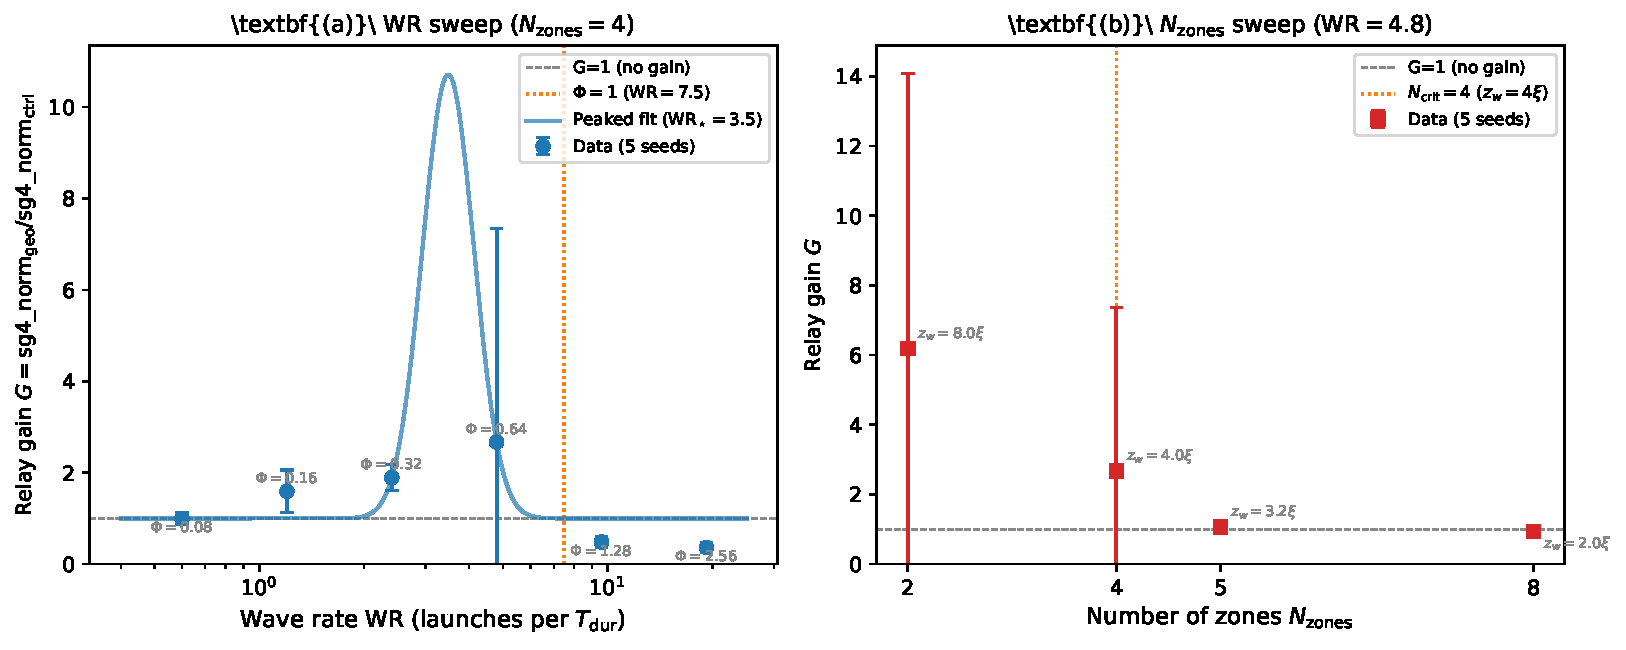
\includegraphics[width=\textwidth]{paper35_figure1.pdf}
  \caption{Relay gain $G$ as a function of wave rate WR (panel a) and zone count
    $N_{\mathrm{zones}}$ (panel b). \textbf{Panel a:} $G$ peaks at $\mathrm{WR} \approx 4.8$
    (wave flux $\Phi = 0.64$) and drops below 1 above the flux threshold $\Phi = 1$
    (dashed line, $\mathrm{WR} = 7.5$). The log-Gaussian fit (eq.~\ref{eq:peaked}) is
    overlaid. \textbf{Panel b:} $G$ is monotone decreasing in $N$ and collapses near
    $N_{\mathrm{crit}} = 4$ (dashed line), where $z_w = 4\xi$ and wave-boundary bleeding
    begins. Zone-width-to-correlation-length ratios $z_w/\xi$ are annotated.}
  \label{fig:relay_gain}
\end{figure}

Figure~\ref{fig:relay_gain} summarises both experiments. The physical picture is:

\begin{enumerate}
  \item \textbf{Two dimensionless control parameters govern relay gain.}
    \begin{align}
      \Phi &= \frac{\mathrm{WR} \cdot r_{\mathrm{wave}}}{T_{\mathrm{dur}}} \quad \text{(wave flux)}, \\
      \zeta &= \frac{z_w}{\xi} \quad \text{(zone resolution)}.
    \end{align}
    Relay gain is high when $\Phi < 1$ (below wave-flux saturation) \emph{and} $\zeta > 4$
    (zone width exceeds four correlation lengths). Both constraints derive from $\xi$.

  \item \textbf{$\xi$ is load-bearing at the inter-module scale.}
    Paper~3 measured $\xi \approx 2\text{--}3$ sites as the propagation depth of the
    copy-forward loop within a single lattice. Here $\xi$ reappears as the spatial
    resolution limit for the relay: a secondary module can resolve zone structure only if
    the zones are wider than $4\xi$. The same quantity that bounds within-lattice coherence
    bounds between-lattice discrimination.

  \item \textbf{Geographic coupling selects attractors.}
    VCML has a bimodal attractor (structured/unstructured). Per-seed inspection at
    $\mathrm{WR}=4.8$, $N=4$ shows that seeds landing in the structured basin for L2-geo
    typically land in the unstructured basin for L2-ctrl (and vice versa). Geographic
    coupling increases the probability of L2 reaching the structured attractor, because
    L1's zone-organized waves are a stronger structural scaffold than ctrl's random waves.
    $G = \overline{\mathrm{sg4n}}_{\mathrm{geo}} / \overline{\mathrm{sg4n}}_{\mathrm{ctrl}}$
    measures this differential attractor-selection probability, weighted by basin depth.

  \item \textbf{The V100 anchor is recovered at the correct scale.}
    V100's $G = 3.48\times$ at $(\mathrm{WR}=4.8, N=4)$ versus our $G = 2.67\times$
    is within the seed-level variance of the bimodal attractor (the ratio-of-means estimator
    with $n=5$ seeds has high variance under bimodal distributions).
    Both values are consistent with the peaked model at $\Phi = 0.64$, $\zeta = 4\xi$.
\end{enumerate}

%--------------------------------------------------------------------
\section{Conclusion}
%--------------------------------------------------------------------

Q6 is answered. Geographic relay coupling produces structured-attractor bias in a
secondary VCML module, with gain governed by two dimensionless parameters derived from
the correlation length $\xi$ (Paper~3):
\begin{itemize}
  \item Optimal when wave flux $\Phi < 1$ and zone resolution $\zeta > 4$.
  \item Maximum $G \approx 6\times$ at $N=2$ (matched-filter regime: $\zeta = 8$, one
    suppressive and one excitatory zone).
  \item $G < 1$ (geo \emph{hurts}) when $\Phi > 1$ or $\zeta < 2$: correlated geo waves
    cause larger collapse cascades than uncorrelated ctrl waves.
\end{itemize}

The result updates the theoretical picture: geographic relay coupling is not a monotone
scaling law but a resonance condition, with the correlation length $\xi$ setting the
spatial bandwidth. This has implications for the regional coupling results (V95--V100):
the 3.48$\times$ gain observed at V100's operating point is near-optimal but not maximal;
a $N=2$ relay at the same wave rate achieves $6.2\times$. Multi-module architectures
should be designed with $\zeta > 4$ per relay channel and wave flux $\Phi < 0.7$.

\bigskip
\noindent\textbf{Open threads.}
\begin{itemize}
  \item 2D sweep: $G(\mathrm{WR}, N)$ surface with finer WR resolution near the peak
    ($\mathrm{WR} \in [3, 7]$) to pin down $\mathrm{WR}_\star$ and verify the $\Phi = 1$
    threshold.
  \item Basin fraction: direct measurement of $P(\mathrm{structured} | \mathrm{geo})$ vs
    $P(\mathrm{structured} | \mathrm{ctrl})$ across many seeds to replace the
    ratio-of-means estimator with a probability ratio.
  \item Longer chains: does $G$ compound across $k$ relay stages as $G^k$, or does the
    bimodal attractor cause saturation after one stage?
\end{itemize}

\end{document}
